% \documentclass[table]{beamer}
\documentclass[table,handout]{beamer}
\setbeameroption{show notes}
% \setbeameroption{hide notes}
% \setbeameroption{show only notes}
\usepackage{varwidth}

\newif\ifhide
\newif\ifpost
\newif\ifhideclicker

% \hidetrue
% \hideclickertrue
% \posttrue

\newcommand{\whiteout}[1]{\textcolor{white}{#1}}
% \newcommand{\whiteoutbox}[1]{\fcolorbox{white}{white}{\parbox{\dimexpr \linewidth-2\fboxsep-2\fboxrule}{\whiteout{#1}}}}
% \newcommand{\notebox}[1]{\fcolorbox{blue}{white}{\parbox{\dimexpr \linewidth-2\fboxsep-2\fboxrule}{#1}}}
\newcommand{\whiteoutbox}[1]{\fcolorbox{white}{white}{\parbox{\linewidth}{\whiteout{#1}}}}
\newcommand{\notebox}[1]{\fcolorbox{blue}{white}{\parbox{\linewidth}{#1}}}
\newcommand{\blankbox}[1]{\phantom{\varwidth{\linewidth}\whiteoutbox{#1}\endvarwidth}}
\newcommand{\blank}[1]{\phantom{\varwidth{\linewidth}#1\endvarwidth}}

\ifhide%
    \newcommand{\hmask}[1]{\blank{#1}}%
\else%
    \newcommand{\hmask}[1]{#1}%
\fi

\ifhide%
    \newcommand{\wout}[1]{\whiteout{#1}}%
\else%
    \newcommand{\wout}[1]{#1}%
\fi

\ifhide%
    \newcommand{\hignore}[1]{}%
\else%
    \newcommand{\hignore}[1]{#1}%
\fi

\ifpost%
    \newcommand{\nopost}[1]{}%
\else%
    \newcommand{\nopost}[1]{#1}%
\fi

\ifhideclicker%
    \newcommand{\clickerslide}[1]{\stepcounter{clickerQuestionCounter}%
        \begin{frame}[t]
            \textcolor{blue}{Q \arabic{clickerQuestionCounter}:}
        \end{frame}}
\else%
    \newcommand{\clickerslide}[1]{#1}%
\fi

\ifhide%
    \newcommand{\hidebox}[1]{\blank{#1}}%
\else%
    \newcommand{\hidebox}[1]{\notebox{#1}}%
\fi

\ifhide%
    \newcommand{\wbox}[1]{\whiteoutbox{#1}}%
\else%
    \newcommand{\wbox}[1]{\notebox{#1}}%
\fi

\ifhide%
    \newcommand{\nbox}[1]{\blankbox{#1}}%
\else%
    \newcommand{\nbox}[1]{\notebox{#1}}%
\fi

\ifhideclicker%
    \newcommand{\clickeranswer}[1]{#1}%
\else%
    \ifhide%
        \newcommand{\clickeranswer}[1]{#1}%
    \else%
        \newcommand{\clickeranswer}[1]{\textbf{\textcolor{blue}{#1}}}%
    \fi
\fi

\usepackage{beamerthemesplit}
% \usetheme{boxes}
\usetheme{Malmoe}
\usecolortheme{seahorse}
% \usecolortheme{seagull}
\usepackage{ifthen}
\usepackage{xspace}
\usepackage{multirow}
\usepackage{multicol}
\usepackage{booktabs}
\usepackage{xcolor}
\usepackage{wasysym}
\usepackage{comment}
\usepackage{hyperref}
\hypersetup{pdfborder={0 0 0}, colorlinks=true, urlcolor=blue, linkcolor=blue, citecolor=blue}
\usepackage{changepage}
\usepackage[compatibility=false]{caption}
\captionsetup[figure]{font=scriptsize, labelformat=empty, textformat=simple, justification=centering, skip=2pt}
\usepackage{tikz}
\usetikzlibrary{trees,calc,backgrounds}

\usepackage[bibstyle=joaks-slides,maxcitenames=3,mincitenames=1,backend=biber]{biblatex}

\newrobustcmd*{\shortfullcite}{\AtNextCite{\renewbibmacro{title}{}\renewbibmacro{in:}{}\renewbibmacro{number}{}}\fullcite}

\newrobustcmd*{\footlessfullcite}{\AtNextCite{\renewbibmacro{title}{}\renewbibmacro{in:}{}}\footfullcite}

% Make all footnotes smaller
% \renewcommand{\footnotesize}{\scriptsize}

\definecolor{myGray}{gray}{0.9}
\colorlet{rowred}{red!30!white}

\setbeamertemplate{blocks}[rounded][shadow=true]

\setbeamercolor{defaultcolor}{bg=structure!30!normal text.bg,fg=black}
\setbeamercolor{block body}{bg=structure!30!normal text.bg,fg=black}
\setbeamercolor{block title}{bg=structure!50!normal text.bg,fg=black}

\newenvironment<>{varblock}[2][\textwidth]{%
  \setlength{\textwidth}{#1}
  \begin{actionenv}#3%
    \def\insertblocktitle{#2}%
    \par%
    \usebeamertemplate{block begin}}
  {\par%
    \usebeamertemplate{block end}%
  \end{actionenv}}

\newenvironment{displaybox}[1][\textwidth]
{
    \centerline\bgroup\hfill
    \begin{beamerboxesrounded}[lower=defaultcolor,shadow=true,width=#1]{}
}
{
    \end{beamerboxesrounded}\hfill\egroup
}

\newenvironment{onlinebox}[1][4cm]
{
    \newbox\mybox
    \newdimen\myboxht
    \setbox\mybox\hbox\bgroup%
        \begin{beamerboxesrounded}[lower=defaultcolor,shadow=true,width=#1]{}
    \centering
}
{
    \end{beamerboxesrounded}\egroup
    \myboxht\ht\mybox
    \raisebox{-0.25\myboxht}{\usebox\mybox}\hspace{2pt}
}

\newenvironment{mydescription}{
    \begin{description}
        \setlength{\leftskip}{-1.5cm}}
    {\end{description}}

\newenvironment{myitemize}{
    \begin{itemize}
        \setlength{\leftskip}{-.3cm}}
    {\end{itemize}}

% footnote without a marker
\newcommand\barefootnote[1]{%
  \begingroup
  \renewcommand\thefootnote{}\footnote{#1}%
  \addtocounter{footnote}{-1}%
  \endgroup
}

% define formatting for footer
\newcommand{\myfootline}{%
    {\it
    \insertshorttitle
    \hspace*{\fill} 
    \insertshortauthor, \insertshortinstitute
    % \ifx\insertsubtitle\@empty\else, \insertshortsubtitle\fi
    \hspace*{\fill}
    \insertframenumber/\inserttotalframenumber}}

% set up footer
\setbeamertemplate{footline}{%
    \usebeamerfont{structure}
    \begin{beamercolorbox}[wd=\paperwidth,ht=2.25ex,dp=1ex]{frametitle}%
        % \Tiny\hspace*{4mm}\myfootline\hspace{4mm}
        \tiny\hspace*{4mm}\myfootline\hspace{4mm}
    \end{beamercolorbox}}

% remove navigation bar
\beamertemplatenavigationsymbolsempty

\makeatletter
    \newenvironment{noheadline}{
        \setbeamertemplate{headline}[default]
        \def\beamer@entrycode{\vspace*{-\headheight}}
    }{}
\makeatother

\newcounter{clickerQuestionCounter}
\ifhideclicker%
\newenvironment{clickerquestion}
{ \stepcounter{clickerQuestionCounter}
  \begin{enumerate}[Q \arabic{clickerQuestionCounter}:]\color{white} }
{ \end{enumerate} }
\else%
\newenvironment{clickerquestion}
{ \stepcounter{clickerQuestionCounter}
  \begin{enumerate}[Q \arabic{clickerQuestionCounter}:] }
{ \end{enumerate} }
\fi

\ifhideclicker%
\newenvironment{clickeroptions}
{ \begin{enumerate}[\begingroup\color{white} 1)\endgroup]\color{white} }
{ \end{enumerate} }
\else%
\newenvironment{clickeroptions}
{ \begin{enumerate}[\begingroup\color{red} 1)\endgroup] }
{ \end{enumerate} }
\fi


\tikzstyle{centered} = [align=center, text centered, font=\sffamily\bfseries]
\tikzstyle{skip} = [centered, inner sep=0pt, fill]
\tikzstyle{empty} = [centered, inner sep=0pt]
\tikzstyle{inode} = [centered, circle, minimum width=4pt, fill=black, inner sep=0pt]
\tikzstyle{tnode} = [centered, circle, inner sep=1pt]
\tikzset{
  % edge styles
  level distance=10mm,
  mate/.style={edge from parent/.style={draw,distance=3pt}},
  mleft/.style={grow=left, level distance=10mm, edge from parent path={(\tikzparentnode.west)--(\tikzchildnode.east)}},
  mright/.style={grow=right, level distance=10mm, edge from parent path={(\tikzparentnode.east)--(\tikzchildnode.west)}},
  % node styles
  male/.style={rectangle,minimum size=4mm,fill=gray!80},
  female/.style={circle,minimum size=4mm,fill=gray!80},
  amale/.style={male,fill=red},
  afemale/.style={female,fill=red},
}

\newcommand{\highlight}[1]{\textcolor{violet}{\textit{\textbf{#1}}}}
\newcommand{\super}[1]{\ensuremath{^{\textrm{\sffamily #1}}}}
\newcommand{\sub}[1]{\ensuremath{_{\textrm{\sffamily #1}}}}
\newcommand{\dC}{\ensuremath{^\circ{\textrm{C}}}}
\newcommand{\tb}{\hspace{2em}}
\providecommand{\e}[1]{\ensuremath{\times 10^{#1}}}
\newcommand{\myHangIndent}{\hangindent=5mm}

\newcommand{\spp}[1]{\textit{#1}}

\newcommand\mybullet{\leavevmode%
\usebeamertemplate{itemize item}\hspace{.5em}}

\makeatletter
\newcommand*{\rom}[1]{\expandafter\@slowromancap\romannumeral #1@}
\makeatother

\newcommand{\blankslide}{{\setbeamercolor{background canvas}{bg=black}
\setbeamercolor{whitetext}{fg=white}
\begin{frame}<handout:0>[plain]
\end{frame}}}

\newcommand{\whiteslide}{
\begin{frame}<handout:0>[plain]
\end{frame}}

\newcommand{\f}[1]{\ensuremath{F_{#1}}}
\newcommand{\x}[1]{X\ensuremath{^{#1}}}
\newcommand{\y}[1]{Y\ensuremath{^{#1}}}

% Population growth macros
\newcommand{\popsize}[1]{\ensuremath{N_{#1}}}
\newcommand{\popgrowthratediscrete}[1]{\ensuremath{\lambda_{#1}}}
\newcommand{\popgrowthrate}[1]{\ensuremath{r_{#1}}}
\newcommand{\ptime}{\ensuremath{t}\xspace}

\tikzset{hide on/.code={\only<#1>{\color{white}}}}
\tikzset{
    invisible/.style={opacity=0},
    visible on/.style={alt={#1{}{invisible}}},
    alt/.code args={<#1>#2#3}{%
        \alt<#1>{\pgfkeysalso{#2}}{\pgfkeysalso{#3}}
        % \pgfkeysalso doesn't change the path
    },
}

\bibliography{../bib/references}
\author[J.\ Oaks]{
    %Jamie R.\ Oaks\inst{1}
    Jamie R.\ Oaks
}
\institute[BIOL 180]{
    \inst{}%
        BIOL 180: Introductory Biology
}



\title[Disease ecology]{Disease ecology}
% \date{\today}
\date{May 19, 2015}

% \setbeamertemplate{section in toc}[sections numbered]
% \setbeamertemplate{subsection in toc}[subsections numbered]

\begin{document}

\begin{noheadline}
\maketitle
\end{noheadline}

\nopost{
\begin{noheadline}
\begin{frame}[c]
    \vspace{-6mm}
    \begin{center} 
        \includegraphics[height=1.2\textheight]{../images/seating-chart-2.pdf}
    \end{center}
\end{frame}
\end{noheadline}
}

% \clickerslide{
% \begin{noheadline}
% \begin{frame}[t]
%     \begin{adjustwidth}{-2em}{-1.5em}
%         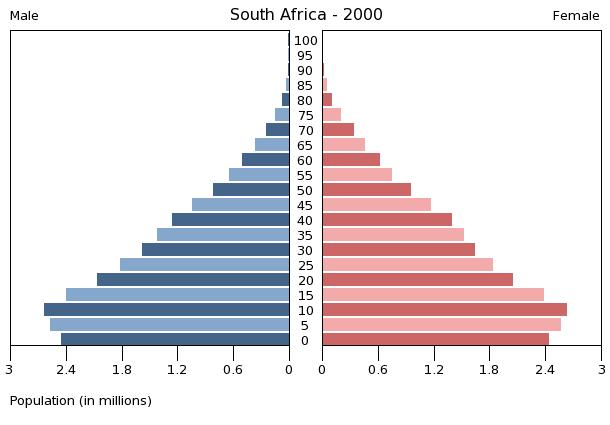
\includegraphics[width=0.5\linewidth]{age-pyramid-south-africa-2000.png}
%         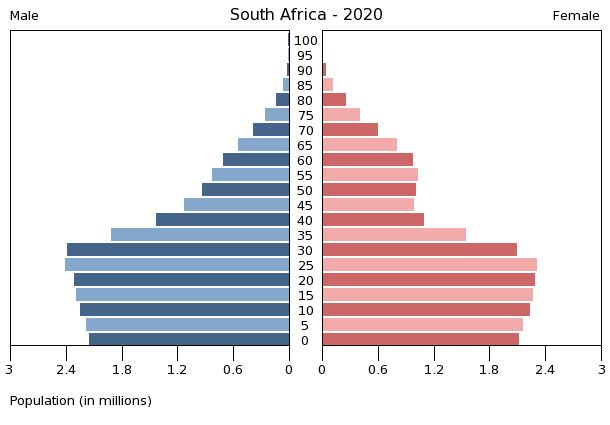
\includegraphics[width=0.5\linewidth]{age-pyramid-south-africa-2020.png}
%     \begin{clickerquestion}
%         \item Data from the same population of long-lived organisms, 20 years
%             apart. Which of the following conclusions is NOT valid? 

%         \begin{clickeroptions}
%             \item \clickeranswer{Over this interval, maximum lifespan in males
%                     becomes $>$10 years longer than maximum lifespan in
%                     females.}
%             \item A catastrophic event wiped out many females who were in their
%                 20s during the first time interval.
%             \item Population growth rate is just becoming stabilized in the
%                 left graph; it is declining in the right graph. 
%             \item At both times, the sex ratio at birth is even or very
%                 slightly male-biased.
%         \end{clickeroptions}
%     \end{clickerquestion}
%     \end{adjustwidth}
%     \note[item]{This is human population of South Africa in 2000 and 2020}
% \end{frame}
% \end{noheadline}
% }

\clickerslide{
\begin{noheadline}
\begin{frame}
    \begin{adjustwidth}{-2em}{-1.5em}
    \begin{columns}

    \column{0.42\linewidth}

    \begin{clickerquestion}
        \item This population pyramid is from China, 1990. During Mao's Great
            Leap Forward (1958--1961), tens of millions of people died of
            starvation over a 3--4 year period. Which interval on the graph
            identifies when it occurred?
        \begin{clickeroptions}
            \item 1
            \item \clickeranswer{2}
            \item 3
            \item 4
            \item China's population is so large that
                the impact is not visible.
        \end{clickeroptions}
    \end{clickerquestion}
    \nbox{\tiny NOTE, we see the impact from the decrease in fertility during
        the famine (not the people that died from famine).}

    \column{0.58\linewidth}

    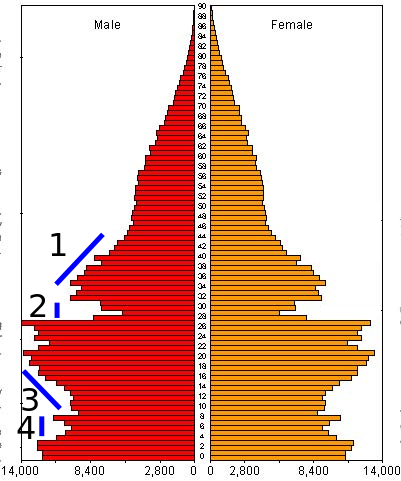
\includegraphics[width=\columnwidth]{age-pyramid-china-1990.png}

    \end{columns}

    \end{adjustwidth}
    \note[item]{Would not see impact on population growth curve. Age pyramid
        gives more detail by plotting age classes.}
\end{frame}
\end{noheadline}
}

\begin{noheadline}
\begin{frame}
\frametitle{Today's issues:}
\vspace{5mm}
% \tableofcontents[subsectionstyle=hide]
\tableofcontents
\end{frame}
\end{noheadline}

\section[How do coevolutionary arms races work?]{How do coevolutionary arms
    races work?}

\begin{frame}[t]
    \begin{adjustwidth}{-2em}{-1.5em}
        How do coevolutionary arms races work?

        \vspace{2mm}
        Malaria as a model

        \begin{itemize}
            \item<2-> Malaria is a disease caused by 4 species of
                \textit{Plasmodium} parasites

                \vspace{5mm}
            \item<2-> Kills $\approx$1 million people per year

                \vspace{5mm}
            \item<2-> Sickens $\approx$300 million people per year

                \vspace{5mm}
            \item<2-> \textit{Plasmodium} cells are passed from infected
                mosquitoes to humans, and from infected humans to mosquitoes
        \end{itemize}
    \end{adjustwidth}
    \note[item]{Mortality is equivalent to 8 747s, loaded with passengers,
        crashing every day}
    \note[item]{Morbidity is roughly equal to the U.S.\ population}
    \note[item]{Why aren't physicians and drug companies doing more?}
    \note[item]{Role of Gates Foundation}
\end{frame}

\begin{frame}[t]
    \begin{adjustwidth}{-2em}{-1.5em}
        Arms race I: Malaria and public health officials

        \begin{itemize}
            \item<2-> Use of DDT to kill mosquitoes:

                \nbox{Very effective at first, but now widespread resistance to
                    DDT in mosquito populations}

                \vspace{5mm}
            \item<2-> Chloroquine, mefloquine, other quinine-derived drugs:

                \nbox{Widespread resistance to quinine-derived drugs in
                    \textit{Plasmodium} populations (also, expensive and nasty
                    side effects)}

                \vspace{5mm}
            \item<2-> Current emphasis: use of insecticide-impregnated bed nets
                (most mosquitoes bite at night)---why effective?

                \nbox{Reduce transmission rates to reduce \textit{Plasmodium}
                    population; ``physical'' defense to which neither
                    mosquitoes nor \textit{Plasmodium} has heritable variation
                    for resistance.}
        \end{itemize}
    \end{adjustwidth}
\end{frame}

\begin{frame}[t]
    \begin{adjustwidth}{-2em}{-1.5em}
        Arms race II: Evolutionary responses in humans

        \begin{itemize}
            \item<2-> Hemoglobin (Hb) is a protein that carries oxygen in red
                blood cells; the normal allele is Hb$A$

            \item<2-> The sickling allele (Hb$S$) gives protection against
                \textit{Plasmodium} in heterozygotes

            \item<2-> Hb$S$ causes sickle cell disease in homozygotes

        \end{itemize}

        \uncover<3->{
        \vspace{-1mm}
        \begin{table}%[htbp]
            \centering
            \begin{tabular}{ R{3cm} | C{2cm} | C{2cm} |C{2cm} |}
                \multicolumn{1}{c}{} &
                \multicolumn{1}{c}{$AA$} &
                \multicolumn{1}{c}{$AS$} &
                \multicolumn{1}{c}{$SS$} \\
                \cline{2-4}
                Anemia & \cmask{none} & \cmask{mild} & \cmask {severe} \\
                \cline{2-4}
                Malaria protection & \cmask{susceptible} & \cmask{protection} & \cmask {protection} \\
                \cline{2-4}
            \end{tabular}
        \end{table}

        \vspace{3mm}
        Question: In areas with and without malaria, does natural selection
        favor individuals with Hb$S$ allele?

        \nbox{Where malaria is absent, Hb$S$ will have low fitness and be at
            very low frequency. Where malaria is present, Hb$S$ allele will
            have higher fitness and will increase in frequency.}
        } 

    \end{adjustwidth}
\end{frame}

\begin{frame}[t]
    \begin{adjustwidth}{-2em}{-1.5em}
    Recent data: study Hb alleles in healthy and \textit{Plasmodium}-infected
    people from Burkina Faso.

    \begin{itemize}
        \item<1-> Observe relatively high frequency of Hb$C$ allele
    \end{itemize}

    \begin{enumerate}
        \item<2-> In healthy people, Hb$C$ genotypes are in Hardy-Weinberg
            proportions.

            \vspace{2mm}
        \item<2-> Among \textit{Plasmodium}-infected people, observe
            \highlight{ALMOST NO} Hb$CC$ genotypes
    \end{enumerate}

    \uncover<2->{
    Interpret observations 1 \& 2:

    \nbox{Given $CC$ is in HW proportion among healthy people, and is absent
        (NOT in HW proportions) from infected people, individuals with the $CC$
        genotype do not appear to be getting sick (protected from
        \textit{Plasmodium})!}
    }
    \barefootnote{\shortfullcite{Modiano2001}}
    \end{adjustwidth}
    \note[item]{Hb$C$ exclusively in northern savannas of Western Africa}
\end{frame}

\begin{frame}[t]
    \begin{adjustwidth}{-2em}{-1.5em}
        \begin{itemize}
            \item Estimate: Risk of infection reduced by 29\% in Hb$AC$
                individuals and by 93\% in Hb$CC$ individuals.

                \vspace{1mm}
            \item Very little adverse affects in $AC$ and $CC$ individuals.
            
                \vspace{1mm}
            \item How is selection acting on Hb$C$ alleles (what do you predict
                will happen to the frequency of Hb$C$ in Burkina Faso
                population)?

                \nbox{Should see rapid increases in the frequency of Hb$C$ in
                    these populations over time.}

                \vspace{3mm}
            \item<2-> Note: Follow-up studies in Ghana and Mali showed mixed
                results about whether Hb$C$ offered protection from infection
                or only prevented disease.
            
            \begin{itemize}
                \item<2-> Why might results differ in different populations?

                    \nbox{Mixed results in other populations is likely due to
                        different strains of \textit{Plasmodium}}
            \end{itemize}

        \end{itemize}

        \barefootnote{\tiny \shortfullcite{Mockenhaupt2004};
            \shortfullcite{Agarwal2000}}
    \end{adjustwidth}
\end{frame}

\section[Can parasites manipulate their hosts?]{Can parasites manipulate their
    hosts?}

\begin{frame}[t]
    \begin{adjustwidth}{-2em}{-1.5em}
        Can parasites manipulate their hosts?

        \vspace{2mm}
        Does natural selection favor alleles that allow parasites to manipulate
        host behavior in a way that increases their transmission to new hosts? 

        \uncover<2->{
        \vspace{2mm}
        Host manipulation by \textit{Plasmodium}? 
        }

        \uncover<3->{
        \begin{itemize}
            \item 19 human volunteers (Tanzania); each individual has unique
                genetic traits that allow identification of blood

                \vspace{4mm}
            \item Assign volunteers randomly to sleep in the same houses

                \vspace{4mm}
            \item Collect mosquitoes the following day
        \end{itemize}
        }

        \barefootnote{\shortfullcite{Koella1998}}
    \end{adjustwidth}
\end{frame}

\begin{frame}[t]
    \begin{adjustwidth}{-2em}{-1.5em}
        \vspace{-2mm}
        The data:

        \vspace{-3mm}
        \begin{table}%[htbp]
            \centering
            \begin{tabular}{ L{3.3cm} | C{3cm} | C{3cm} | C{1.2cm} }
                \multicolumn{1}{c}{} &
                \multicolumn{1}{c}{Bit $>$ than 1 person} &
                \multicolumn{1}{c}{Bit 1 person} &
                \multicolumn{1}{c}{Total} \\
                \cline{2-3}
                Mosquito infected & \cmask{20} & \cmask{69} & 89 \\
                \cline{2-3}
                Mosquito uninfected & \cmask{17} & \cmask{156} & 173\\
                \cline{2-3}
            \end{tabular}
        \end{table}

        \begin{table}%[htbp]
            \centering
            \begin{tabular}{ L{3.3cm} | C{3cm} | C{3cm} | C{1.2cm} }
                \multicolumn{1}{c}{} &
                \multicolumn{1}{c}{Fully fed} &
                \multicolumn{1}{c}{Half fed} &
                \multicolumn{1}{c}{Total} \\
                \cline{2-3}
                Mosquito infected & \cmask{229} & \cmask{51} & 280 \\
                \cline{2-3}
                Mosquito uninfected & \cmask{1058} & \cmask{424} & 1482 \\
                \cline{2-3}
            \end{tabular}
        \end{table}
        
        \vspace{2mm}
        What statistical test should be used?

        \nbox{Goodness-of-fit test (e.g., chi-square test)}

        P-value = 0.007 (top) and 0.0004 (bottom); What do you conclude about
        whether \textit{Plasmodium} can manipulate mosquitoes?

        \nbox{\scriptsize These data strongly support the hypothesis
            \textit{Plasmodium} can manipulate mosquito behavior. More
            specifically, the data support that \textit{Plasmodium} makes
            mosquitoes feed more and from more individuals.}

        \barefootnote{\shortfullcite{Koella1998}}
    \end{adjustwidth}
\end{frame}

\begin{frame}[t]
    \begin{adjustwidth}{-2em}{-1.5em}
        \textit{Plasmodium} manipulation \ldots additional findings:

        \begin{itemize}
            \item<2-> \textit{Plasmodium} suppresses feeding of infected
                mosquitoes before the parasites are mature (i.e., before they
                can be transmitted to humans), and increases mosquito feeding
                once they are mature

                \begin{itemize}
                    \item Why would the suppression of biting be adaptive?

                        \nbox{Biting is risky for mosquitoes. By preventing the
                            mosquito from biting until the parasites are ready
                            to be transmitted, the parasites increase the
                            probability they will infect humans before the
                            mosquito gets squashed!}
                \end{itemize}

                \vspace{4mm}
            \item<3-> \textit{Plasmodium} makes humans more attractive to
                infected and uninfected mosquitoes, ONLY when the parasites are
                ready to be transmitted to the mosquito
        \end{itemize}
    \end{adjustwidth}
\end{frame}

\begin{frame}[t]
    \begin{adjustwidth}{-2em}{-1.5em}
        When you sneeze, is your body ridding itself of viruses/bacteria, or is
        the virus/bacterium manipulating you to increase transmission to new
        hosts?

        \vspace{3mm}
        \begin{itemize}
            \item How would you test your hypothesis?
        \end{itemize}

        \vspace{9mm}
        Does the flu make you more social?

        \vspace{3mm}
        \begin{itemize}
            \item How would you test this hypothesis?
        \end{itemize}

        \nbox{Reiber et al.\ 2010 compared the behavior of participants for
            48-hours before and after flu shot. Participants interacted with
            significantly more people during the 48-hours after the shot.}

        \barefootnote{\shortfullcite{Reiber2010}}
    \end{adjustwidth}
\end{frame}

\clickerslide{
\begin{frame}
    \begin{clickerquestion}
        \item \textit{Toxoplasma} is a parasite that infects rats and has to be
            transmitted to cats to complete its life cycle. If
            \textit{Toxoplasma} manipulates rat behavior, how would infected
            vs.\ uninfected rats react to the smell of cat urine? 

        \begin{clickeroptions}
            \item Infected rats have an adverse reaction to cat urine;
                uninfected mice have no reaction.
            \item \clickeranswer{Infected rats are attracted to cat urine;
                    uninfected have an adverse reaction.}
            \item Infected cats should stop hunting rats.
            \item Infected cats should be more motivated to hunt rats.
        \end{clickeroptions}
    \end{clickerquestion}
\end{frame}
}


\section[The evolution of virulence]{The evolution of virulence}

\begin{frame}[t]
    \begin{adjustwidth}{-2em}{-1.5em}
        The evolution of virulence

        \vspace{2mm}
        Under what conditions are parasites expected to evolve to be extremely
        virulent? (virulence = tendency to cause illness/death)

        \begin{itemize}
            \item<2-> Observation 1: Virulence is a function of parasite growth
                rate (number of host cells killed).

                \vspace{5mm}
            \item<3-> Observation 2: The probability of parasite transmission
                at any moment is a function of the number of parasites present.

                \vspace{5mm}
            \item<4-> Observation 3: Host morbidity and mortality is also a
                function of parasite growth rate (number of host cells killed).

                \vspace{5mm}
            \item<5-> Observation 4: There is heritable variation in degree of
                virulence (it can respond to selection).
        \end{itemize}

    \end{adjustwidth}
\end{frame}

\clickerslide{
\begin{frame}
    \begin{clickerquestion}
        \item Under what conditions are parasites expected to evolve to be
            extremely virulent? 

        \begin{clickeroptions}
            % \item In emerging (new) diseases. This is because over time,
            %     parasites evolve to become benign. (It is not favorable for
            %     parasites to kill their host.)
            \item When transmission rates to new hosts are low (i.e.,
                opportunities for transmission are rare).
            \item \clickeranswer{When transmission rates to new hosts are high
                    (i.e., opportunities for transmission are common).}
            \item When the parasite is a specialist (has only one host
                species). 
            \item When the parasite is a generalist (has many host species). 
        \end{clickeroptions}
    \end{clickerquestion}
\end{frame}
}

\section[Environmental disturbance and infectious disease]{How are
    human-induced changes in the environment affecting infectious disease?}

\begin{frame}[t]
    \begin{adjustwidth}{-2em}{-1.5em}
        How are human-induced changes in the environment affecting infectious
        disease?

        \vspace{2em}
        Two examples of medical ecology:

        \begin{enumerate}
            \item Survey of incidence of cholera bacterium in waters
                off Peru
        \end{enumerate}

    \end{adjustwidth}
\end{frame}

\begin{frame}[t]
    \begin{adjustwidth}{-2em}{-1.5em}
        \vspace{-3mm}
        What is the relationship between seawater temperature and
        \textit{Vibrio cholerae} infection rate?

        \centering{
            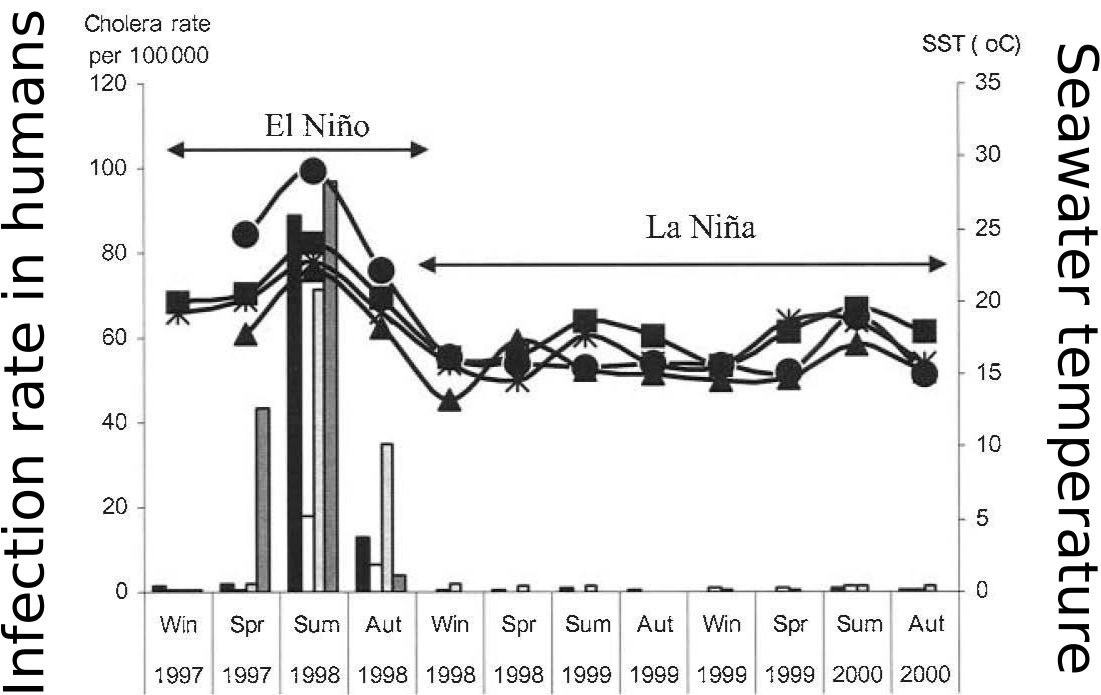
\includegraphics[width=0.82\linewidth]{vibrio-data.png}}

        \vspace{-2mm}
        \barefootnote{\tiny\shortfullcite{Gil2004}}
    \end{adjustwidth}
\end{frame}

\begin{frame}[t]
    \begin{adjustwidth}{-2em}{-1.5em}
        \vspace{-3mm}
        \begin{columns}[t]

            \column{0.74\linewidth}

            \vspace{-4mm}
            \begin{enumerate}
                \addtocounter{enumi}{1}
                \item Investigating Lyme disease in humans
            \end{enumerate}

            \vspace{1mm}
            {\small
                How is the incidence of Lyme disease changing in this region?

                    \nbox{\scriptsize It is increasing}

                Do the data support the traditional hypothesis that Lyme
                disease incidence is controlled by deer population density?

                    \nbox{\scriptsize No. The abundance of deer is not changing
                        (or slightly declining) while the incidence of the
                        disease is increasing}

                Mice also host the bacterium that causes Lyme disease.  Fox eat
                mice. Coyotes eat fox.  How do these observations help explain
                the data?

                    \nbox{\scriptsize The increase in coyotes is causing a
                        decline in foxes. This could be causing an increase in
                        mouse populations, which in turn is increasing the rate
                        of transmission to humans}

                What environmental changes by humans would explain these data?

                    \nbox{\scriptsize Humans have removed top predators, like
                        wolves, that would compete with, and eat, coyotes.} }


            \column{0.25\linewidth}

            \vspace{-3mm}
            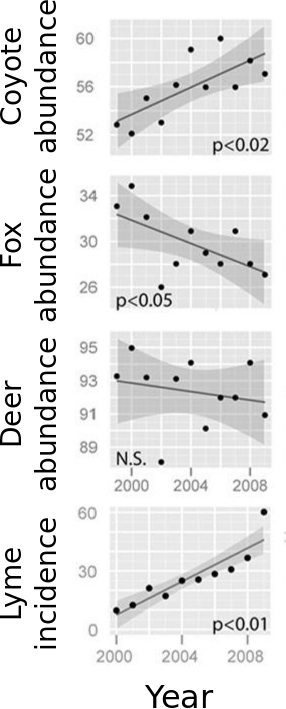
\includegraphics[width=\columnwidth]{lyme-dz.png}

        \end{columns}

        \vspace{-4mm}
        \barefootnote{\tiny\shortfullcite{Levi2012}}
    \end{adjustwidth}
\end{frame}

\end{document}

\clickerslide{
\begin{frame}
    \begin{clickerquestion}
        \item 
        \begin{clickeroptions}
            \item 
            \item 
            \item 
            \item 
        \end{clickeroptions}
    \end{clickerquestion}
\end{frame}
}

\clickerpost{
{
\usebackgroundtemplate{\includegraphics[page=17,width=\paperwidth]{./24-Radiation-extinction.pdf}}
\begin{frame}[t,plain]
    \begin{adjustwidth}{-2em}{-1.5em}
        \cmask{Answer: 3}
    \end{adjustwidth}
\end{frame}
}
}

